\section{Data}
\label{sec:data}

We use four image populations, all built on Euclid Q1 VIS
images~\citep{euclidq1overview, euclidq1data}: simulated lenses with matched negatives, which
form the labelled source; expert-graded real lenses; an unlabelled pool of real Euclid
galaxies; and objects graded X (not a lens) by experts, used as hard negatives.
Figure~\ref{fig:setup} shows how they are split.

\subsection{Arc-on-real simulations}

Only the arc is simulated. Each positive is a real Euclid VIS cutout of a galaxy, the
deflector, with a ray-traced arc painted on. The deflectors are Q1 catalogue galaxies whose
stored values satisfy $\log M_* \geq \DeflMassFloor{}$ and
$\DeflZmin{} \leq z_{\rm phot} \leq \DeflZmax{}$~\citep{euclidq1phz}. From a pool of
\rwDeflPool{} such galaxies, about \rwDeflArc{} can produce an arc with Einstein radius
$\theta_{\rm E} \geq 0.75''$. We generated 30\,000 lenses from this pool, reusing a deflector
for up to \rwDeflReuse{} lenses; the 24\,000 training lenses sit on \rwDeflDistinct{} distinct
galaxies. Painting
onto real cutouts keeps the real line-of-sight objects, noise and point-spread function, which
is standard practice~\citep{holismokesXI, lines2025discoveryengineC, unions2025}; our lensed
sources are parametric models (Section~\ref{sec:sim-pipeline}).

Each simulated lens is paired with the same galaxy without an arc, so within a pair only the
arc differs. The training set as a whole is not paired this way. Only $\rvBareDeflN{}$ of the
$\rvSourceNegN{}$ negatives are bare deflectors, while every positive sits on a galaxy with
$\log M_* \geq \DeflMassFloor{}$, so the appearance of a massive galaxy could act as a class
cue. We checked the cues we could measure: no single stored brightness, redshift or mass
variable separates the training positives from the negatives, with AUROC between
$\rvHostAurocMin{}$ and $\rvHostAurocMax{}$. Stellar mass and redshift are stored only for
the deflectors, so this check covers brightness alone for the random-galaxy and grade-X
negatives, and we did not test morphology.

An earlier, fully synthetic generator had no deflector light and let a classifier separate
the classes by brightness, which is why we moved to painting arcs onto real galaxies.

\subsection{The simulation pipeline}
\label{sec:sim-pipeline}

We assigned each deflector a velocity dispersion $\sigma_v$ by abundance matching, derived
the Einstein radius $\theta_E$ from $\sigma_v$ under a singular isothermal ellipsoid (SIE),
and drew the source redshift so that $\theta_E$ fell in an acceptable range given the
deflector's photometric redshift~\citep{euclidq1phz}. Sources are parametric models (single
S\'ersic or bulge-plus-disk) fitted to COSMOS F814W galaxies of the $I < \simSourceSample$
sample~\citep{mandelbaum2014great3}, drawn with GalSim~\citep{rowe2015galsim} through
\texttt{COSMOSCatalog} with \texttt{gal\_type="\simSourceGalType"}, and kept if their
half-light radius lay between $\simSourceHlrMin''$ and $\simSourceHlrMax''$. We ray-traced each
source through the SIE with \texttt{lenstronomy}~\citep{birrer2018lenstronomy,
birrer2021lenstronomy}, convolved it with a Gaussian PSF of FWHM $0.16''$, scaled it so that
its brightest arc pixel reached a signal-to-noise ratio drawn uniformly between
\simArcSnrMin{} and \simArcSnrMax{}, and added it to the cutout without further noise, since
the cutout already carries real Euclid noise. The output
is 30\,000 lenses and 30\,000 matched non-lenses at $64 \times 64$ pixels and $0.1''$/pixel.

The velocity dispersions follow the SDSS early-type velocity dispersion function
of~\citet{choi2007vdf},
\begin{equation}
  \frac{\mathrm{d}n}{\mathrm{d}\sigma} \;\propto\;
  \left(\frac{\sigma}{\sigma_*}\right)^{\alpha}
  \exp\!\left[-\left(\frac{\sigma}{\sigma_*}\right)^{\beta}\right] \frac{1}{\sigma},
  \label{eq:vdf}
\end{equation}
with $\sigma_* = 161$\,km\,s$^{-1}$, $\alpha = 2.32$ and $\beta = 2.67$ on
$\sigma \in [80, 400]$\,km\,s$^{-1}$, assigned to deflectors by stellar-mass rank under a
fixed seed. We use these central stellar dispersions directly as SIE dispersions, and we apply
this $z \lesssim 0.1$ function to every deflector without redshift evolution.

Every image enters the encoder through one fixed transformation: a per-image clip at the 0th
and 99.7th percentiles, a rescale to $[0,1]$ and an $\operatorname{arcsinh}$ stretch, resized
to $224 \times 224$ (Appendix~\ref{app:repro} gives its provenance). When an arm trains on
images, we flip each image horizontally and vertically at random, rotate it by a random angle
between $-\augRotDeg{}^\circ$ and $+\augRotDeg{}^\circ$, filling the corners with zeros, and
shift it by up to $\pm \augShiftPx{}$ pixels, equally for all classes; random centroid shifts
stop a lens finder learning the image centre as a feature~\citep{holismokesXI}. The strong
view that FreeMatch uses also zooms by \augZoomLo{}--\augZoomHi{} and, half the time, erases a
random patch covering \augEraseLoPct{}--\augEraseHiPct{}\% of the image. Test images are not
augmented.

\subsection{Real lenses and the unlabelled pool}

The positive class is 489 real lenses from the Euclid Q1 Discovery Engine catalogue, 246 of
grade A and 243 of grade B~\citep{discoveryengineA}, with their cutouts from the catalogue's
data record~\citep{discoveryenginecat}. Experts graded each image A (confident lens), B
(probable), C (possible) or X (not a lens); grades A and B are cuts on an expert score, above 2
and above 1.5~\citep[Sect.~6.2]{discoveryengineA}. We follow the benchmark and use grades A and B as
positives~\citep{lines2025simstosky}. The catalogue lists 497 grade A/B systems; eight are
missing from our processed set because their files were absent from, or failed to read in,
the released archives, leaving 489.

The unlabelled pool is about 225\,000 Euclid VIS cutouts of objects selected from the MER
catalogue by VIS PSF flux between \FluxMin{} and \FluxMax{}~$\mu$Jy ($I_E \approx \MagFaint{}$
to $\MagBright{}$ in PSF magnitude)~\citep{euclidq1mer}, with a VIS detection, positive
near-infrared fluxes, a point-like probability below 0.3, an extended probability above 0.5
and a spurious probability below 0.3. The query was capped at 250\,000 rows with no ordering,
so the pool is the archive's first matches rather than a random draw. We assign objects to
roles by a hash of their identifier and draw each role with a fixed seed. Separately, \GradeXUsed{}
of the \GradeXAll{} objects graded X in version 0.0.1 of the Discovery Engine
catalogue~\citep{discoveryenginecat001} (those whose cutouts we could recover from the
image tiles our pipeline downloaded; we did not record why each of the others was dropped)
enter the source negatives as hard negatives; later
versions publish grades A--C only~\citep{discoveryenginecat}, and \GradeXnowC{} of these
objects are graded C in version 0.0.3. They appear in training only.

\subsection{Splits and fold rotation}
\label{sec:splits}

One splits file, built deterministically under seed 42, fixes every membership.
\emph{Source-train} holds 24\,000 simulated positives against 24\,000 negatives: the \GradeXUsed{}
grade-X objects, 2881 bare deflectors and 16\,664 random galaxies. We split the simulated
lenses 80/20 into training and validation grouped by deflector, because one deflector hosts up
to ten lenses; \citep{astrovink} guard against the same leak for reused deflectors with a
perceptual-hashing check. \emph{Source-validation} holds the other 6000 positives
against 6000 negatives. With no real labels for selection, held-out source data is the only
proxy, and a weak one~\citep{musgrave2021realitycheck}.

\emph{Target} rotates. For fold $k$ it is the graded lenses of the other four folds, about 391,
together with about 391 random galaxies drawn fresh for that fold. We balance it 1:1 because
under differing class proportions, aligning feature distributions is not guaranteed to help and
can increase target error~\citep{zhao2019invariant, zhao2020gls, classimbalanceda}; Section~\ref{sec:labels} gives the reason we chose
it and how its labels are used. Any two folds share $\rvSharedTargetMin{}$ to
$\rvSharedTargetMax{}$ of their target lenses (Section~\ref{sec:intervals}).

Our second experiment (Section~\ref{sec:dilute-methods}) uses a diluted target. Each fold keeps
the same \dlPoolLens{} target lenses (\dlPoolLensFour{} on fold 4) and holds galaxies up to
exactly \dlRatio{} times as many: the fold's existing target galaxies first, then fresh draws
from the target partition. The \dlFresh{} fresh galaxies were screened by exact Euclid ID against
every split role, the catalogued grade A and B lenses, the simulation hosts and the grade-X
objects, and none of them is a catalogued lens, a simulation host or a grade-X object, or holds
another split role. The existing galaxies include simulation hosts
already counted in the leakage audit below (\dlHosts{} on folds 1--4); the fresh draws contain
none. The first part of that experiment's pre-registration fixes this construction
(Appendix~\ref{sec:hashes}).

\emph{Test} is per fold: that fold's 98 held-out graded lenses (97 on fold 4) against one
shared pool of \TestNegDOne{} random galaxies (\TestNegDrawn{} as drawn, less the
\DOneRemoved{} we excluded; Section~\ref{sec:testpool}). The test negatives were selected by
catalogue cuts and hash-based sampling alone. One shared pool keeps the FPR${}=10^{-3}$
threshold fixed across folds. The benchmark's non-lens sample is limited at
$I_E < 22.5$~\citep{lines2025simstosky}; ours extends to $\MagFaint{}$ in PSF magnitude, and
\FracFaintTest{}\% of our test negatives are fainter than 22.5, so the two pools are not
matched in depth. We divided the 489 lenses into five folds stratified by grade; each lens is
tested exactly once.

\subsection{Leakage audit}

Our split-building script enforces nine groups of rules before it writes the file
(Appendix~\ref{sec:splitrules}). We then checked the splits again, in the spirit of the
leakage taxonomy of Kapoor and Narayanan~\citep{kapoor2023}. Perceptual hashing of the 489
lenses flagged eight similar pairs; all are more than 3900 arcseconds apart and are distinct
systems. Matching by exact Euclid ID, rebuilt from coordinates because some stored
identifiers are rounded, found that \DOneLensNeg{} catalogued lenses and \DOneDeflNeg{}
simulation hosts were among the test negatives, all of them random-galaxy draws, and
\DeflOtherNeg{} more simulation hosts among the training, validation and target negatives, in
their random-galaxy draws and among the grade-X hard negatives. The bare-deflector negatives
are simulation hosts by design and are not counted. Section~\ref{sec:testpool} gives what we
did about the test pool.

\begin{figure}[t]
\centering
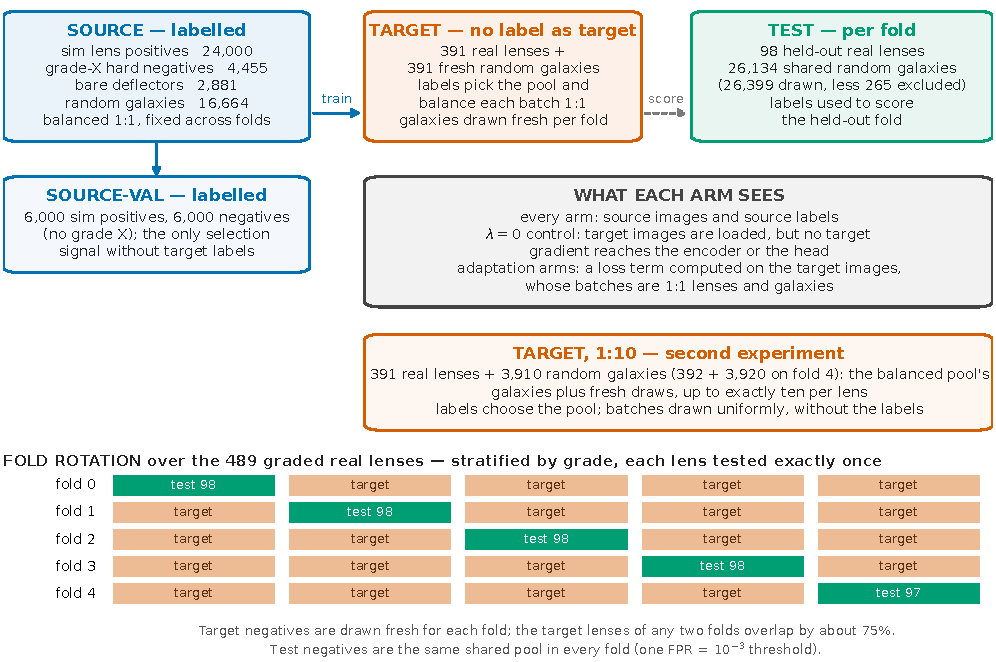
\includegraphics[width=\textwidth]{F1_setup_v6.pdf}
\caption{\textbf{Data roles and fold rotation.} Counts are read from the splits file and, for
the 1:10 target, from its pool file; test negatives are counted after the exclusion of
Section~\ref{sec:testpool}. Target negatives are drawn fresh for each fold; the target lenses of
any two folds overlap by about \rvTargetOverlapPct{}\%. In the main design the catalogue labels
choose the target pool and balance each target batch (Section~\ref{sec:labels}); they are never
a training target. The bottom box is the 1:10 target of the second experiment
(Section~\ref{sec:dilute-methods}): the labels still choose its pool, and its batches are drawn
uniformly, without the labels.}
\label{fig:setup}
\end{figure}

\begin{figure}[t]
\centering
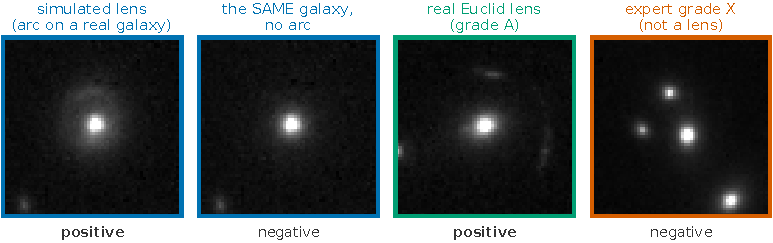
\includegraphics[width=\textwidth]{F2_cutouts.pdf}
\caption{\textbf{One example from each population}, under the per-image stretch the encoder
receives: a simulated lens at the median Einstein radius of its simulation batch, the same
galaxy with no arc,
the grade-A lens at the median expert score, and a grade-X hard negative. Image credit: ESA
Euclid/Euclid Consortium/NASA/Q1-2025.}
\label{fig:cutouts}
\end{figure}
